\documentclass{article}
\usepackage{fancyhdr}
\usepackage[margin=1in]{geometry}
\usepackage{amsmath}
\usepackage{siunitx}
\usepackage{array}
\usepackage{pgfplots}
\usepackage{graphicx}
\usepackage{circuitikz}


\pagestyle{fancy}
\fancyhf{}
\chead{Física Experimental III • Experimento realizado em 20/10/2023}
\rfoot{\thepage}
\renewcommand{\headrulewidth}{0.4pt}

\begin{document}

\begin{center}
    \huge
    \textbf{Tensões e Correntes Elétricas}
    \normalsize
    \vspace{10pt}

    Matheus Aparecido Souza Silva, Isabela Sant'Ana, Gustavo Peres, João Vitor Costa
    \vspace{5pt}

    \textbf{Turma}: TA \quad \textbf{Horário}: 6M45 \quad \textbf{Curso}: Engenharia Elétrica
\end{center}

\section{Coleta de dados:}

\subsection{Tabela de dados das medições de resistências}

\begin{tabular}{|c|c|c|c|}
    \hline
    Associação & Valor Nominal (\(\Omega\)) $\pm$ Tolerância & Valor Experimental (\(\Omega\)) $\pm$ Incerteza \\
    \hline
    R\textsubscript{1} & 47 $\pm$ 5\% & 46.70 $\pm$ 0.62 \\
    \hline
    R\textsubscript{2} & 220 $\pm$ 5\% & 218.8 $\pm$ 2.2 \\
    \hline
    R\textsubscript{3} & 120 $\pm$ 5\% & 120.9 $\pm$ 1.3 \\
    \hline
    R\textsubscript{e} (Série) & 387 $\pm$ 5\% & 386.4 $\pm$ 3.7 \\
    \hline
    R\textsubscript{e} (Paralelo) & 29.277 $\pm$ 5\% & 29.20 $\pm$ 0.46 \\
    \hline
    R\textsubscript{e} (Misto) & 94.935 $\pm$ 5\% & 94.9 $\pm$ 1.0 \\
    \hline 
\end{tabular}

\subsection{Tabela de dados experimentais}

\begin{tabular}{|c|c|c|c|c|}
    \hline
     & Resistores Individuais & Resistores em Série & Resistores em Paralelo & Associação Mista \\
    \hline
    $V_1 \pm \Delta V_1$ & $4.024 \pm 0.022$ & $0.491 \pm 0.004$ & $4.025 \pm 0.022 $ & $0.491 \pm 0.004 $\\
    \hline
    $V_2 \pm \Delta V_2$ & $4.028 \pm 0.022$ & $2.321 \pm 0.013$ & $4.029 \pm 0.022 $ & $3.544 \pm 0.019 $\\
    \hline
    $V_3 \pm \Delta V_3$ & $4.029 \pm 0.022$ & $1.223 \pm 0.008$ & $4.026 \pm 0.022 $ & $3.544 \pm 0.019 $\\
    \hline
    $V \pm \Delta V$ & $---$ & $4.035 \pm 0.022$ & $4.026 \pm 0.022 $ & $4.035 \pm 0.022 $\\
    \hline
    $i_1 \pm \Delta i_1$ & $0.087 \pm 0.004$ & $0.011 \pm 0.003$ & $0.086 \pm 0.004$ & \\
    \hline
    $i_2 \pm \Delta i_2$ & $0.018 \pm 0.003$ & $0.011 \pm 0.003$ & $0.019 \pm 0.003$ & \\
    \hline
    $i_3 \pm \Delta i_3$ & $0.035 \pm 0.003$ & $0.011 \pm 0.003$ & $0.036 \pm 0.003$ & \\
    \hline
    $i \pm \Delta i$ & $---$ & $0.011 \pm 0.003$ &$0.141 \pm 0.005$ & \\
    \hline
    $R_1 \pm \Delta R_1$ & $46.242 \pm 2.141$ & $44.63 \pm 12.178$ &$46.802 \pm 2.191$ & \\
    \hline
    $R_2 \pm \Delta R_2$ & $223.5 \pm 37.270$ & $211 \pm 57.546$ &$212.052 \pm 33.502$ & \\
    \hline
    $R_3 \pm \Delta R_3$ & $114.971 \pm 9.874$ & $118.18 \pm 32.240$ & $111.916 \pm 9.346$ & \\
    \hline
    $R_e \pm \Delta R_e$ & $---$ & $366.818 \pm 100.061$ & $28.553 \pm 1.069$ & \\
    \hline
\end{tabular}

\section{Atividades} 

\subsection{Associação de resistores em série:}

\begin{figure}[h]
    \centering
    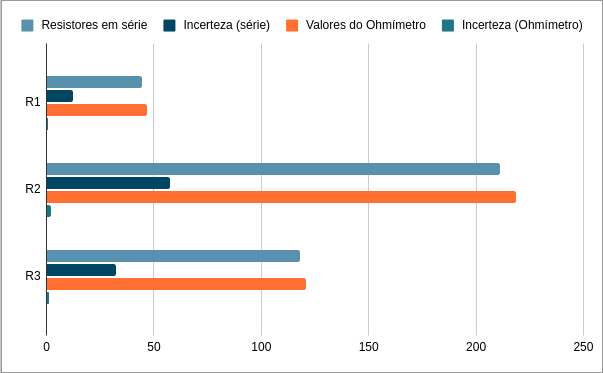
\includegraphics[width=0.5\textwidth]{Associação dos resistores em série.png}
  \end{figure}

\subsubsection{Verificação da Lei das Malhas em Resistores em Série}
A Lei das Malhas é um princípio fundamental em circuitos elétricos que estabelece que a soma das quedas de tensão em um circuito fechado (malha) é igual à fem da fonte de tensão. Para validar a Lei das Malhas, realizamos a análise das medições das quedas de tensão em resistores em série, levando em conta as incertezas associadas.

Os valores das quedas de tensão (\(V_1\), \(V_2\), e \(V_3\)) foram obtidos a partir das medições experimentais, conforme apresentado na tabela de dados experimentais. Para a configuração de resistores em série, temos:

\begin{align*}
V_1 \pm \Delta V_1 &= 0.491 \pm 0.004 \, \text{V} \\
V_2 \pm \Delta V_2 &= 2.321 \pm 0.013 \, \text{V} \\
V_3 \pm \Delta V_3 &= 1.223 \pm 0.008 \, \text{V}
\end{align*}

Agora, somamos as quedas de tensão, considerando as incertezas:

\begin{align*}
V_1 + V_2 + V_3 &= (0.491 \pm 0.004) \, \text{V} + (2.321 \pm 0.013) \, \text{V} + (1.223 \pm 0.008) \, \text{V} \\
&= 4.035 \pm 0.025 \, \text{V}
\end{align*}

A fem fornecida pela fonte de tensão foi medida como \(4.025 \pm 0.022\) V. Comparando a soma das quedas de tensão com a fem:

\begin{align*}
E &= 4.025 \pm 0.022 \, \text{V}
\end{align*}

Observamos que a soma das quedas de tensão em resistores em série (\(4.035 \pm 0.025\) V) está dentro do intervalo da fem (\(4.025 \pm 0.022\) V) fornecida pela fonte de tensão. Portanto, concluímos que a Lei das Malhas é satisfeita, e a análise das medições corrobora esse princípio fundamental em circuitos elétricos.

\subsection{Associação de resistores em paralelo:}

\begin{figure}[h]
    \centering
    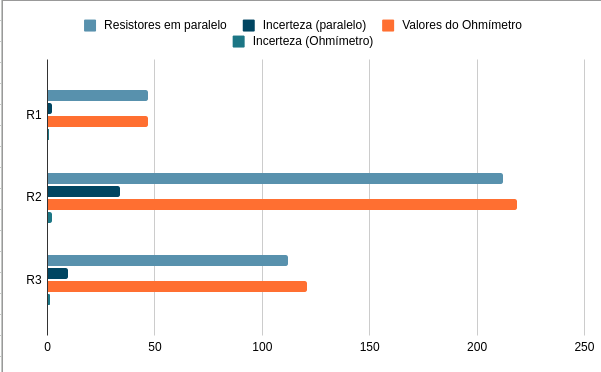
\includegraphics[width=0.5\textwidth]{Associação de resistores em paralelo.png}
  \end{figure}

\subsubsection{Verificação da Lei dos Nós em Resistores em Paralelo}
A Lei dos Nós é um princípio fundamental em circuitos elétricos que estabelece que a soma das correntes que entram em um nó (ponto de conexão) é igual à soma das correntes que saem do nó. Para validar a Lei dos Nós, realizamos a análise das medições das correntes em resistores em paralelo, levando em conta as incertezas associadas.

Na tabela de dados experimentais, os valores relacionados aos resistores em paralelo são os seguintes:

\begin{align*}
i_1 \pm \Delta i_1 &= 0.086 \pm 0.004 \, \text{A} \\
i_2 \pm \Delta i_2 &= 0.019 \pm 0.003 \, \text{A} \\
i_3 \pm \Delta i_3 &= 0.036 \pm 0.003 \, \text{A} \\
i \pm \Delta i &= 0.141 \pm 0.005 \, \text{A} \quad \text{(corrente total medida na saída da fonte de tensão)}
\end{align*}

A Lei dos Nós estabelece que a soma das correntes que entram em um nó é igual à soma das correntes que saem do nó. Portanto, a soma das correntes em cada resistor em paralelo deve ser igual à corrente total medida na saída da fonte de tensão, levando em consideração as incertezas.

Vamos verificar isso calculando a soma das correntes em cada resistor em paralelo:

\begin{align*}
i_1 + i_2 + i_3 &= (0.086 \pm 0.004) \, \text{A} + (0.019 \pm 0.003) \, \text{A} + (0.036 \pm 0.003) \, \text{A} \\
&= 0.141 \pm 0.010 \, \text{A}
\end{align*}

Agora, você pode comparar essa soma com a corrente total medida na saída da fonte de tensão:

\begin{align*}
i \pm \Delta i &= 0.141 \pm 0.005 \, \text{A}
\end{align*}

Observamos que a soma das correntes em resistores em paralelo (\(0.141 \pm 0.010\) A) está dentro do intervalo da corrente total medida na saída da fonte de tensão (\(0.141 \pm 0.005\) A). Portanto, concluímos que a Lei dos Nós é satisfeita, e a análise das medições corrobora esse princípio fundamental em circuitos elétricos.

\section{Associação mista}

\begin{center}
    \begin{circuitikz}
        \draw (0,0) to[battery1, v=$V$] (0,3);
        \draw (0,3) to[R, l=$R1$] (2,3);
        \draw (2,3) to[short, *-] (2,4);
        \draw (2,4) to[R, l=$R2$] (4,4);
        \draw (2,3) to[short, *-] (2,2);
        \draw (2,2) to[R, l=$R3$] (4,2);
        \draw (4,4) to[short, -*] (4,2);
        \draw (4,2) to[short, -*] (4,0);
        \draw (4,0) to[short] (0,0);
      \end{circuitikz}
       
\end{center}

  

\end{document}